\chapter{Matchings}
\section{Introduction}
% 7.1 Motivation
\topic{Motivation}
Imagine a group of people has to split up in pairs and take part in a competition. Every person has several people they'd be happy to compete with, and we assume this is symmetric.
This situation can be modeled using a graph. How would a possible matching look like which would please everyone?

Example:
\begin{center}
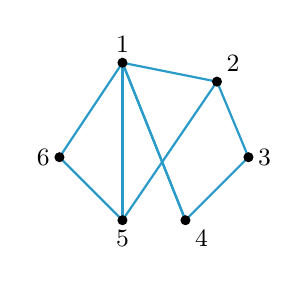
\begin{tikzpicture}[scale=0.8]
    % Coordinates matching the visual layout (1 top, 2 top-right, 3 right, 4 bottom-right, 5 bottom, 6 left)
    \coordinate (n1) at (0, 1.5);
    \coordinate (n2) at (1.5, 1.2);
    \coordinate (n3) at (2, 0);
    \coordinate (n4) at (1, -1);
    \coordinate (n5) at (0, -1);
    \coordinate (n6) at (-1, 0);

    % Edges
    \draw[cyan!80!black, thick] (n6)--(n1)--(n2)--(n3)--(n4)--(n1)--(n5)--(n6); % Outer cycle-ish
    \draw[cyan!80!black, thick] (n1)--(n5);
    \draw[cyan!80!black, thick] (n1)--(n4);
    \draw[cyan!80!black, thick] (n2)--(n5);

    % Labels
    \foreach \i in {1,2,3,4,5,6} \filldraw (n\i) circle (2pt);
    \node[above] at (n1) {\small 1}; \node[above right] at (n2) {\small 2};
    \node[right] at (n3) {\small 3}; \node[below right] at (n4) {\small 4};
    \node[below] at (n5) {\small 5}; \node[left] at (n6) {\small 6};
\end{tikzpicture}
\end{center}

Possible matchings are

\begin{center}
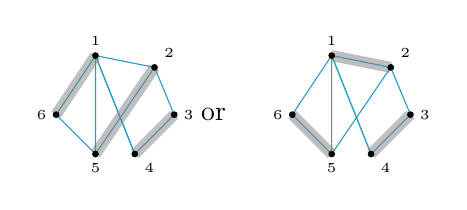
\begin{tikzpicture}[scale=0.5]
    % Left Matching
    \begin{scope}[xshift=0cm]
        \coordinate (n1) at (0, 1.5); \coordinate (n2) at (1.5, 1.2); \coordinate (n3) at (2, 0);
        \coordinate (n4) at (1, -1); \coordinate (n5) at (0, -1); \coordinate (n6) at (-1, 0);
        
        \draw[cyan!80!black] (n6)--(n1)--(n2)--(n3)--(n4)--(n1)--(n5)--(n6);
        \draw[cyan!80!black] (n1)--(n5); \draw[cyan!80!black] (n1)--(n4); \draw[cyan!80!black] (n2)--(n5);
        
        % Thick Matching Edges (Grey highlight style)
        % Notes show: (1-6), (2-5), (3-4)
        \draw[line width=4pt, gray, opacity=0.5] (n1)--(n6);
        \draw[line width=4pt, gray, opacity=0.5] (n2)--(n5);
        \draw[line width=4pt, gray, opacity=0.5] (n3)--(n4);
        
        \foreach \i in {1,...,6} \filldraw (n\i) circle (2pt);
        \node[above] at (n1) {\tiny 1}; \node[above right] at (n2) {\tiny 2}; \node[right] at (n3) {\tiny 3};
        \node[below right] at (n4) {\tiny 4}; \node[below] at (n5) {\tiny 5}; \node[left] at (n6) {\tiny 6};
    \end{scope}

    \node at (3, 0) {or};

    % Right Matching
    \begin{scope}[xshift=6cm]
        \coordinate (n1) at (0, 1.5); \coordinate (n2) at (1.5, 1.2); \coordinate (n3) at (2, 0);
        \coordinate (n4) at (1, -1); \coordinate (n5) at (0, -1); \coordinate (n6) at (-1, 0);
        
        \draw[cyan!80!black] (n6)--(n1)--(n2)--(n3)--(n4)--(n1)--(n5)--(n6);
        \draw[cyan!80!black] (n1)--(n5); \draw[cyan!80!black] (n1)--(n4); \draw[cyan!80!black] (n2)--(n5);
        
        % Thick Matching Edges
        % Notes show: (2-5), (1-4)
        \draw[line width=4pt, gray, opacity=0.5] (n2)--(n1);
        \draw[line width=4pt, gray, opacity=0.5] (n3)--(n4);
        \draw[line width=4pt, gray, opacity=0.5] (n5)--(n6);

        \foreach \i in {1,...,6} \filldraw (n\i) circle (2pt);
        \node[above] at (n1) {\tiny 1}; \node[above right] at (n2) {\tiny 2}; \node[right] at (n3) {\tiny 3};
        \node[below right] at (n4) {\tiny 4}; \node[below] at (n5) {\tiny 5}; \node[left] at (n6) {\tiny 6};
        
    \end{scope}
\end{tikzpicture}
\end{center}
If we pair 2 with 5 3 and 4 with 1, this is still a matching.\\

\begin{center}
    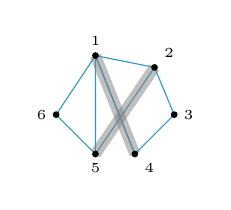
\begin{tikzpicture}[scale=0.5]
        \coordinate (n1) at (0, 1.5); \coordinate (n2) at (1.5, 1.2); \coordinate (n3) at (2, 0);
        \coordinate (n4) at (1, -1); \coordinate (n5) at (0, -1); \coordinate (n6) at (-1, 0);
        
        \draw[cyan!80!black] (n6)--(n1)--(n2)--(n3)--(n4)--(n1)--(n5)--(n6);
        \draw[cyan!80!black] (n1)--(n5); \draw[cyan!80!black] (n1)--(n4); \draw[cyan!80!black] (n2)--(n5);
        
        % Thick Matching Edges
        % Notes show: (2-5), (1-4)
        \draw[line width=4pt, gray, opacity=0.5] (n2)--(n5);
        \draw[line width=4pt, gray, opacity=0.5] (n1)--(n4);
        
        \foreach \i in {1,...,6} \filldraw (n\i) circle (2pt);
        \node[above] at (n1) {\tiny 1}; \node[above right] at (n2) {\tiny 2}; \node[right] at (n3) {\tiny 3};
        \node[below right] at (n4) {\tiny 4}; \node[below] at (n5) {\tiny 5}; \node[left] at (n6) {\tiny 6};
    \end{tikzpicture}
\end{center}
But we have 2 happy teams and can't form another one. It is not perfect...

Observation: The goal will be to pick a set of edges which do not share end vertices.

% 7.2 Definition
\begin{definition}
Let $G$ be any graph.
\begin{enumerate}
    \item[i)] A \textbf{\color{red}matching} for $G$ is a set $M \subseteq E(G)$ of pairwise disjoint edges.
    \item[ii)] $v \in V(G)$ is called \textbf{\color{red}$M$-saturated} if exists $e \in M$ s.t. $v \in e$ (i.e. if it is the endpoint of some edge in $M$). Otherwise, we call $v$ \textbf{\color{red}$M$-unsaturated}.
    \item[iii)] We call a matching $M$ \textbf{\color{red}maximal} iff $M \cup \{e\}$ is not a matching for any $e \in E(G) \setminus M$.
    \item[iv)] We say that $M$ is a \textbf{\color{red}maximum matching} if it has the largest cardinality among all possible matchings.
    \item[v)] Finally, we call $M$ \textbf{\color{red}perfect} if any $v \in V(G)$ is $M$-saturated.
\end{enumerate}
\end{definition}

% 7.3 Example
\begin{example}
Consider the graph $G =$
\begin{center}
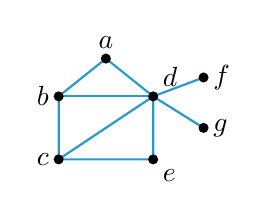
\begin{tikzpicture}[scale=0.8, baseline=(current bounding box.center)]
    % Coordinates matching the handwritten layout
    \coordinate (b) at (0, 1);
    \coordinate (c) at (0, 0);
    \coordinate (e) at (1.5, 0);
    \coordinate (d) at (1.5, 1);
    \coordinate (a) at (0.75, 1.6); % Top peak
    \coordinate (f) at (2.3, 1.3); % Leaf from d
    \coordinate (g) at (2.3, 0.5); % Leaf from e

    % Edges
    \draw[cyan!80!black, thick] (b)--(a)--(d)--(e)--(c)--(b); % Pentagon
    \draw[cyan!80!black, thick] (b)--(d); % Diagonal
    \draw[cyan!80!black, thick] (d)--(f); % Leaf f
    \draw[cyan!80!black, thick] (d)--(g); % Leaf g
    \draw[cyan!80!black, thick] (c)--(d);


    % Nodes and Labels
    \foreach \p/\pos/\label in {a/above/a, b/left/b, c/left/c, d/above right/d, e/below right/e, f/right/f, g/right/g}
        \filldraw (\p) circle (2pt) node[\pos] {$\label$};
\end{tikzpicture}
\end{center}

Then
\begin{center}
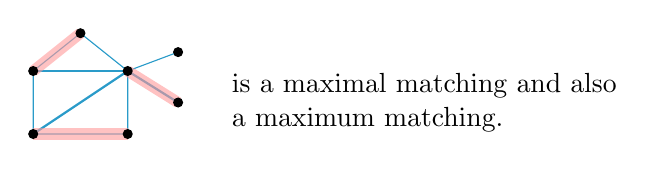
\begin{tikzpicture}[scale=0.8]
    % --- SCENARIO 1: Maximum Matching ---
    \begin{scope}[xshift=0cm]
        \coordinate (b) at (0, 1); \coordinate (c) at (0, 0); \coordinate (e) at (1.5, 0);
        \coordinate (d) at (1.5, 1); \coordinate (a) at (0.75, 1.6);
        \coordinate (f) at (2.3, 1.3); \coordinate (g) at (2.3, 0.5);

        % Base Graph
        \draw[cyan!80!black] (b)--(a)--(d)--(e)--(c)--(b);
        \draw[cyan!80!black] (b)--(d); \draw[cyan!80!black] (d)--(f); \draw[cyan!80!black, thick] (d)--(g); % Leaf g
        \draw[cyan!80!black, thick] (c)--(d);

        % Highlighted Matching {ab, ce, df}
        \draw[line width=4pt, red!40, opacity=0.6] (a)--(b);
        \draw[line width=4pt, red!40, opacity=0.6] (c)--(e);
        \draw[line width=4pt, red!40, opacity=0.6] (d)--(g);

        \foreach \p in {a,b,c,d,e,f,g} \filldraw (\p) circle (2pt);
    \end{scope}
    
    \node[right, align=left] at (3, 0.5) {is a maximal matching and also \\ a maximum matching.};
\end{tikzpicture}
\end{center}

Further,
\begin{center}
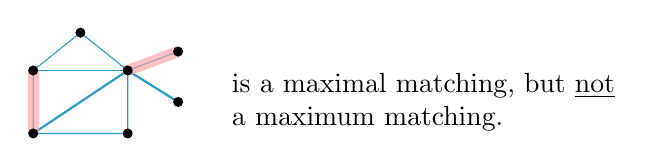
\begin{tikzpicture}[scale=0.8]
    % --- SCENARIO 2: Maximal but NOT Maximum ---
    \begin{scope}[xshift=0cm]
        \coordinate (b) at (0, 1); \coordinate (c) at (0, 0); \coordinate (e) at (1.5, 0);
        \coordinate (d) at (1.5, 1); \coordinate (a) at (0.75, 1.6);
        \coordinate (f) at (2.3, 1.3); \coordinate (g) at (2.3, 0.5);

        \draw[cyan!80!black] (b)--(a)--(d)--(e)--(c)--(b);
        \draw[cyan!80!black] (b)--(d); \draw[cyan!80!black] (d)--(f); \draw[cyan!80!black, thick] (d)--(g); % Leaf g
        \draw[cyan!80!black, thick] (c)--(d);

        % Highlighted Matching {bd, ce}
        \draw[line width=4pt, red!40, opacity=0.6] (b)--(c);
        \draw[line width=4pt, red!40, opacity=0.6] (d)--(f);

        \foreach \p in {a,b,c,d,e,f,g} \filldraw (\p) circle (2pt);
    \end{scope}
    
    \node[right, align=left] at (3, 0.5) {is a maximal matching, but \underline{not} \\ a maximum matching.};
\end{tikzpicture}
\end{center}

Also,
\begin{center}
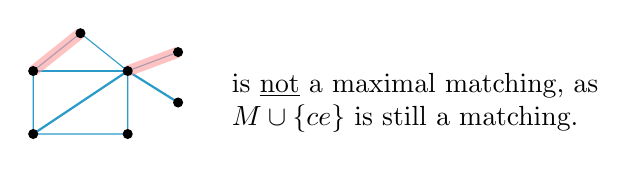
\begin{tikzpicture}[scale=0.8]
    % --- SCENARIO 3: Not Maximal ---
    \begin{scope}[xshift=0cm]
        \coordinate (b) at (0, 1); \coordinate (c) at (0, 0); \coordinate (e) at (1.5, 0);
        \coordinate (d) at (1.5, 1); \coordinate (a) at (0.75, 1.6);
        \coordinate (f) at (2.3, 1.3); \coordinate (g) at (2.3, 0.5);

        \draw[cyan!80!black] (b)--(a)--(d)--(e)--(c)--(b);
        \draw[cyan!80!black] (b)--(d); \draw[cyan!80!black] (d)--(f); \draw[cyan!80!black, thick] (d)--(g); % Leaf g
        \draw[cyan!80!black, thick] (c)--(d);

        % Highlighted Matching {ab, df}
        \draw[line width=4pt, red!40, opacity=0.6] (a)--(b);
        \draw[line width=4pt, red!40, opacity=0.6] (d)--(f);

        \foreach \p in {a,b,c,d,e,f,g} \filldraw (\p) circle (2pt);
    \end{scope}
    
    \node[right, align=left] at (3, 0.5) {is \underline{not} a maximal matching, as \\ $M \cup \{ce\}$ is still a matching.};
\end{tikzpicture}
\end{center}

Finally, there are no perfect matchings as $|V(G)|$ is odd.
\end{example}

% 7.4 Remark
\begin{remark}
\begin{enumerate}
    \item[1)] Any perfect matching is a maximum matching.
    \item[2)] Any maximum matching is maximal.
    \item[3)] If $G$ has a perfect matching, then $|G|$ is even.
\end{enumerate}
Further, any matching $M$ is perfect iff it is a maximum matching iff $|M| = \frac{|V|}{2}$.
\end{remark}

% 7.5 Examples
\begin{example}
\begin{center}

% Define colors and styles
\tikzset{
    vertex/.style={circle, draw, fill=black, inner sep=1.5pt, outer sep=0pt},
    highlight/.style={line width=6pt, violet!40, line cap=round},
    edge/.style={thick},
    label text/.style={font=\itshape\small}
}
\newcommand{\greencheck}{\textcolor{green!60!black}{\Huge\checkmark}}
\newcommand{\redcross}{\textcolor{red}{\Huge$\times$}}

\noindent
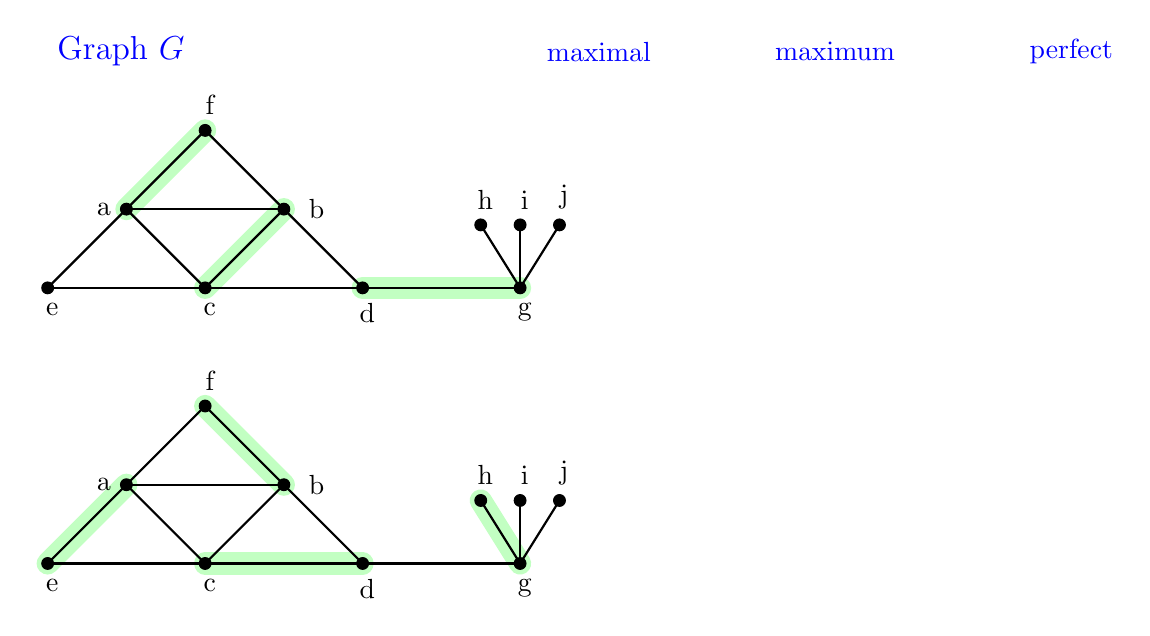
\begin{tikzpicture}[scale=1]

    % --- HEADERS ---
    \node[anchor=west, blue, font=\large] at (0, 3) {Graph $G$};
    \node[blue] at (7, 3) {maximal};
    \node[blue] at (10, 3) {maximum};
    \node[blue] at (13, 3) {perfect};

    % ================= GRAPH 1 (TOP) =================
    \begin{scope}[yshift=0cm]
        % Coordinates
        \coordinate (e) at (0,0);
        \coordinate (c) at (2,0);
        \coordinate (d) at (4,0);
        \coordinate (g) at (6,0);
        \coordinate (a) at (1,1);
        \coordinate (b) at (3,1);
        \coordinate (f) at (2,2);
        \coordinate (h) at (5.5,0.8);
        \coordinate (i) at (6,0.8);
        \coordinate (j) at (6.5,0.8);

        % Highlights (Graph 1)
        \draw[highlight] (a) -- (f);
        \draw[highlight] (c) -- (b);
        \draw[highlight] (d) -- (g);

        % Edges
        \draw[edge] (e)--(c)--(d)--(g);
        \draw[edge] (e)--(a)--(c)--(b)--(d);
        \draw[edge] (a)--(b);
        \draw[edge] (a)--(f)--(b);
        \draw[edge] (g)--(h);
        \draw[edge] (g)--(i);
        \draw[edge] (g)--(j);

        % Nodes and Labels
        \foreach \p/\l/\pos in {e/e/below, c/c/below, d/d/below, g/g/below, a/a/left, b/b/right, f/f/above, h/h/above, i/i/above, j/j/above}
            \node[vertex, label=\pos:{\label t \l}] at (\p) {};

        % Table Marks
        \node at (7, 1) {\greencheck};
        \node at (10, 1) {\redcross};
        \node at (13, 1) {\redcross};
    \end{scope}

    % ================= GRAPH 2 (MIDDLE) =================
    \begin{scope}[yshift=-3.5cm]
        % Coordinates (same as above)
        \coordinate (e) at (0,0);
        \coordinate (c) at (2,0);
        \coordinate (d) at (4,0);
        \coordinate (g) at (6,0);
        \coordinate (a) at (1,1);
        \coordinate (b) at (3,1);
        \coordinate (f) at (2,2);
        \coordinate (h) at (5.5,0.8);
        \coordinate (i) at (6,0.8);
        \coordinate (j) at (6.5,0.8);

        % Highlights (Graph 2)
        \draw[highlight] (e) -- (a);
        \draw[highlight] (f) -- (b);
        \draw[highlight] (c) -- (d);
        \draw[highlight] (h) -- (g);

        % Edges
        \draw[edge] (e)--(c)--(d)--(g);
        \draw[edge] (e)--(a)--(c)--(b)--(d);
        \draw[edge] (a)--(b);
        \draw[edge] (a)--(f)--(b);
        \draw[edge] (g)--(h);
        \draw[edge] (g)--(i);
        \draw[edge] (g)--(j);

        % Nodes and Labels
        \foreach \p/\l/\pos in {e/e/below, c/c/below, d/d/below, g/g/below, a/a/left, b/b/right, f/f/above, h/h/above, i/i/above, j/j/above}
            \node[vertex, label=\pos:{\label t \l}] at (\p) {};

        % Table Marks
        \node at (7, 1) {\greencheck};
        \node at (10, 1) {\greencheck};
        \node at (13, 1) {\redcross};
    \end{scope}

\end{tikzpicture}

\vspace{1em}
\noindent
Note that there can't be a perfect matching, even though $|G|=10$ is even, as any matching uses at most one of $hg, ig$ and $jg$.
\vspace{1em}

\noindent
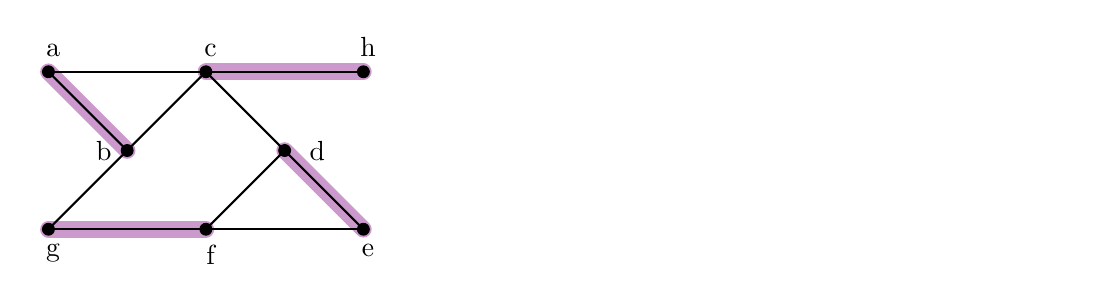
\begin{tikzpicture}[scale=1]
    \tikzset{
        vertex/.style={circle, draw, fill=black, inner sep=1.5pt, outer sep=0pt},
        highlight/.style={line width=6pt, violet!40, line cap=round},
        edge/.style={thick},
        label text/.style={font=\itshape\small}
    }
    
    % ================= GRAPH 3 (BOTTOM) =================
    % Coordinates based on visual layout
    % Bottom row: g, f, e
    \coordinate (g) at (0,0);
    \coordinate (f) at (2,0);
    \coordinate (e) at (4,0);
    % Middle row (bridge): b, d
    \coordinate (b) at (1,1);
    \coordinate (d) at (3,1);
    % Top row: a, c, h
    \coordinate (a) at (0,2);
    \coordinate (c) at (2,2);
    \coordinate (h) at (4,2);

    % Highlights (Graph 3)
    \draw[highlight] (a) -- (b);
    \draw[highlight] (c) -- (h);
    \draw[highlight] (g) -- (f);
    \draw[highlight] (d) -- (e);

    % Edges
    % Vertical/Zigzag stacks
    \draw[edge] (a) -- (b) -- (g);
    \draw[edge] (b) -- (c);
    % Top horizontal
    \draw[edge] (a) -- (c) -- (h);
    % Middle cross connections
    \draw[edge] (c) -- (d);
    \draw[edge] (d) -- (f);
    % Bottom horizontal
    \draw[edge] (g) -- (f) -- (e);
    \draw[edge] (e) -- (d);

    % Nodes and Labels
    \foreach \p/\l/\pos in {g/g/below, f/f/below, e/e/below, b/b/left, d/d/right, a/a/above, c/c/above, h/h/above}
        \node[vertex, label=\pos:{\label t \l}] at (\p) {};

    % Table Marks (Aligned with previous picture coordinates x=7, 10, 13)
    \node at (7, 1) {\greencheck};
    \node at (10, 1) {\greencheck};
    \node at (13, 1) {\greencheck};

\end{tikzpicture}
\end{center}
Note that there can't be a perfect matching, even though $|G|=10$ is even, as any matching uses at most one of $hg, ig$ and $jg$.

We see that while it is rather easy to decide whether a matching is maximal or perfect, things are less clear for a maximum matching. Our next goal is to develop a criterion to help us decide that, called Berge's Theorem.
\end{example}

% 7.6 Definition
\begin{definition}
Let $G$ be a graph and $M$ a matching for $G$ and $p$ a path in $G$.
\begin{enumerate}
    \item[1)] We say that $p$ is \textbf{\color{red}$M$-alternating} if its edges alternate between edges inside and outside $M$.
    \item[2)] We call $p$ \textbf{\color{red}$M$-augmenting} if it is $M$-alternating and its start and end vertex are distinct and both \underline{not} $M$-saturated.
\end{enumerate}
\end{definition}

How does this relate to maximum matchings?

% 7.7 Example
\begin{example}
Consider the graph $G$ with matching $M$ below.
\begin{center}
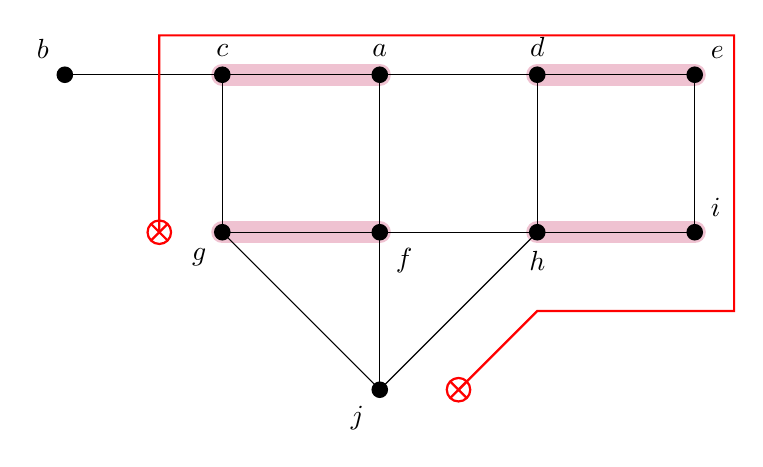
\begin{tikzpicture}[
    scale=1,
    node distance=2cm,
    % Style for the black graph nodes
    vertex/.style={circle, fill=black, inner sep=2pt, minimum size=6pt},
    % Style for the crossed-out red markers
    cut marker/.style={
        circle, draw=red, thick, inner sep=3pt,
        path picture={
            \draw[red, thick] 
            (path picture bounding box.south west) -- (path picture bounding box.north east)
            (path picture bounding box.south east) -- (path picture bounding box.north west);
        }
    }
]

    % --- 1. Define Coordinates ---
    \coordinate (b) at (0, 2);
    \coordinate (c) at (2, 2);
    \coordinate (a) at (4, 2);
    \coordinate (d) at (6, 2);
    \coordinate (e) at (8, 2);

    \coordinate (g) at (2, 0);
    \coordinate (f) at (4, 0);
    \coordinate (h) at (6, 0);
    \coordinate (i) at (8, 0);

    \coordinate (j) at (4, -2);


    % --- 2. Draw Highlights (Purple Lines) ---
    % Drawn first so they appear behind
    \tikzstyle{highlight}=[line width=8pt, purple!40, opacity=0.6, line cap=round]
    
    \draw[highlight] (c) -- (a);
    \draw[highlight] (d) -- (e);
    \draw[highlight] (g) -- (f);
    \draw[highlight] (h) -- (i);


    % --- 3. Draw Black Edges ---
    % Horizontal
    \draw (b) -- (c) -- (a) -- (d) -- (e);
    \draw (g) -- (f) -- (h) -- (i);
    
    % Vertical
    \draw (c) -- (g);
    \draw (a) -- (f);
    \draw (d) -- (h);
    \draw (e) -- (i);
    
    % Triangle connections
    \draw (g) -- (j);
    \draw (f) -- (j);
    \draw (h) -- (j);


    % --- 4. Draw Nodes and Labels ---
    \node[vertex, label=above left:$b$] at (b) {};
    \node[vertex, label=above:$c$] at (c) {};
    \node[vertex, label=above:$a$] at (a) {};
    \node[vertex, label=above:$d$] at (d) {};
    \node[vertex, label=above right:$e$] at (e) {};

    \node[vertex, label=below left:$g$] at (g) {};
    \node[vertex, label=below right:$f$] at (f) {};
    \node[vertex, label=below:$h$] at (h) {};
    \node[vertex, label=above right:$i$] at (i) {};

    \node[vertex, label=below left:$j$] at (j) {};


    % --- 5. Draw the Red Path (Fixed) ---
    % Start point (Left of g)
    \coordinate (start) at (1.2, 0);
    
    % Top boundary box (Above the graph)
    \coordinate (top_left) at (1.2, 2.5);
    \coordinate (top_right) at (8.5, 2.5);
    
    % Bottom boundary path
    % Moved Y to -1.0 so it runs underneath h and f
    \coordinate (btm_right) at (8.5, -1.0); 
    \coordinate (extra) at (6, -1.0); 
    % End point
    % Moved X to 3.0 so it crosses the edge g-j
    \coordinate (end) at (5.0, -2.0);     

    \draw[red, thick] (start) -- (top_left) -- (top_right) -- (btm_right) -- (extra) -- (end);

    \node[cut marker] at (start) {};
    \node[cut marker] at (end) {};

\end{tikzpicture}
\end{center}
The path $p_1 = (g, c, a, d, e, i, h, j)$ is $M$-alternating, but not $M$-augmenting, its start vertex $g$ is $M$-saturated.

On the other hand, the path $p_2 = (b, c, a, d, e, i, h, j)$ is $M$-augmenting. In particular, it is $M$-alternating. What happens if we define a new edge set $M'$ by containing all edges of $M$ outside of $p$ and also exactly those edges of $p$ which were not in $M$?

\begin{center}
    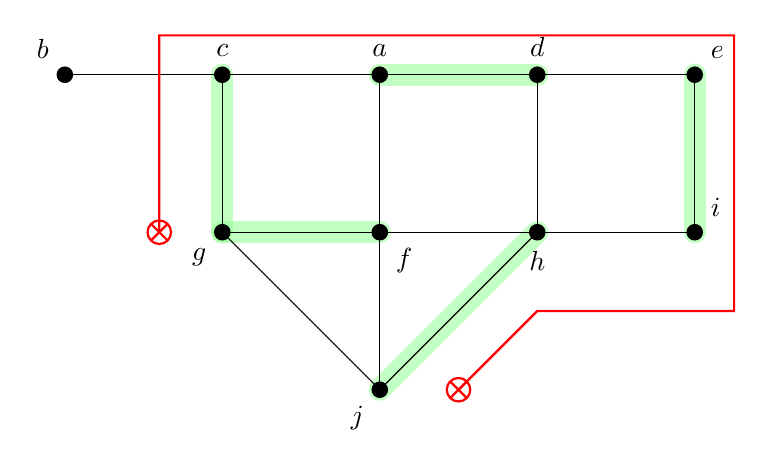
\begin{tikzpicture}[
    scale=1,
    node distance=2cm,
    % Style for the black graph nodes
    vertex/.style={circle, fill=black, inner sep=2pt, minimum size=6pt},
    % Style for the crossed-out red markers
    cut marker/.style={
        circle, draw=red, thick, inner sep=3pt,
        path picture={
            \draw[red, thick] 
            (path picture bounding box.south west) -- (path picture bounding box.north east)
            (path picture bounding box.south east) -- (path picture bounding box.north west);
        }
    }
]

    % --- 1. Define Coordinates ---
    \coordinate (b) at (0, 2);
    \coordinate (c) at (2, 2);
    \coordinate (a) at (4, 2);
    \coordinate (d) at (6, 2);
    \coordinate (e) at (8, 2);

    \coordinate (g) at (2, 0);
    \coordinate (f) at (4, 0);
    \coordinate (h) at (6, 0);
    \coordinate (i) at (8, 0);

    \coordinate (j) at (4, -2);


    % --- 2. Draw Highlights (Purple Lines) ---
    % Drawn first so they appear behind
    \tikzstyle{highlight}=[line width=8pt, green!40, opacity=0.6, line cap=round]
    
    
    \draw[highlight] (c) -- (g);
    \draw[highlight] (d) -- (a);
    \draw[highlight] (g) -- (f);
    \draw[highlight] (h) -- (j);
    \draw[highlight] (i) -- (e);


    % --- 3. Draw Black Edges ---
    % Horizontal
    \draw (b) -- (c) -- (a) -- (d) -- (e);
    \draw (g) -- (f) -- (h) -- (i);
    
    % Vertical
    \draw (c) -- (g);
    \draw (a) -- (f);
    \draw (d) -- (h);
    \draw (e) -- (i);
    
    % Triangle connections
    \draw (g) -- (j);
    \draw (f) -- (j);
    \draw (h) -- (j);


    % --- 4. Draw Nodes and Labels ---
    \node[vertex, label=above left:$b$] at (b) {};
    \node[vertex, label=above:$c$] at (c) {};
    \node[vertex, label=above:$a$] at (a) {};
    \node[vertex, label=above:$d$] at (d) {};
    \node[vertex, label=above right:$e$] at (e) {};

    \node[vertex, label=below left:$g$] at (g) {};
    \node[vertex, label=below right:$f$] at (f) {};
    \node[vertex, label=below:$h$] at (h) {};
    \node[vertex, label=above right:$i$] at (i) {};

    \node[vertex, label=below left:$j$] at (j) {};


    % --- 5. Draw the Red Path (Fixed) ---
    % Start point (Left of g)
    \coordinate (start) at (1.2, 0);
    
    % Top boundary box (Above the graph)
    \coordinate (top_left) at (1.2, 2.5);
    \coordinate (top_right) at (8.5, 2.5);
    
    % Bottom boundary path
    % Moved Y to -1.0 so it runs underneath h and f
    \coordinate (btm_right) at (8.5, -1.0); 
    \coordinate (extra) at (6, -1.0); 
    % End point
    % Moved X to 3.0 so it crosses the edge g-j
    \coordinate (end) at (5.0, -2.0);     

    \draw[red, thick] (start) -- (top_left) -- (top_right) -- (btm_right) -- (extra) -- (end);

    \node[cut marker] at (start) {};
    \node[cut marker] at (end) {};

\end{tikzpicture}
\end{center}

For $p_1=(g,c,a,d,e,i,h,j)$ which was $M$-alternating, but not $M$-augmenting, we obtain an edge set which is \underline{not} a matching.

\begin{center}
    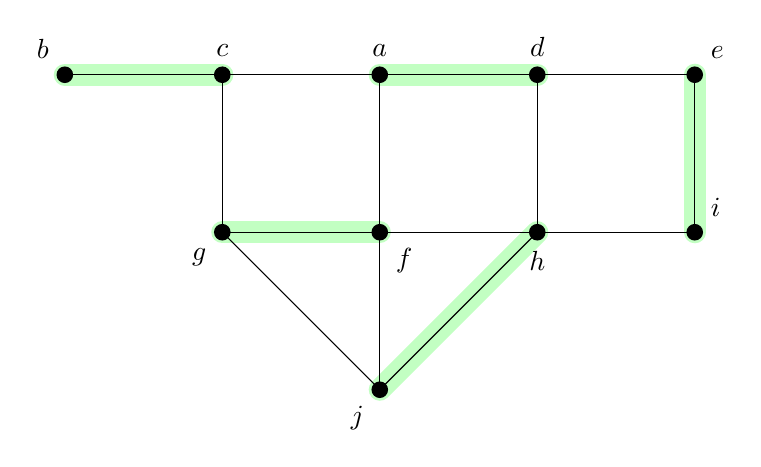
\begin{tikzpicture}[
    scale=1,
    node distance=2cm,
    % Style for the black graph nodes
    vertex/.style={circle, fill=black, inner sep=2pt, minimum size=6pt},
    % Style for the crossed-out red markers
    cut marker/.style={
        circle, draw=red, thick, inner sep=3pt,
        path picture={
            \draw[red, thick] 
            (path picture bounding box.south west) -- (path picture bounding box.north east)
            (path picture bounding box.south east) -- (path picture bounding box.north west);
        }
    }
]

    % --- 1. Define Coordinates ---
    \coordinate (b) at (0, 2);
    \coordinate (c) at (2, 2);
    \coordinate (a) at (4, 2);
    \coordinate (d) at (6, 2);
    \coordinate (e) at (8, 2);

    \coordinate (g) at (2, 0);
    \coordinate (f) at (4, 0);
    \coordinate (h) at (6, 0);
    \coordinate (i) at (8, 0);

    \coordinate (j) at (4, -2);


    % --- 2. Draw Highlights (Purple Lines) ---
    % Drawn first so they appear behind
    \tikzstyle{highlight}=[line width=8pt, green!40, opacity=0.6, line cap=round]
    
    
    \draw[highlight] (c) -- (b);
    \draw[highlight] (d) -- (a);
    \draw[highlight] (g) -- (f);
    \draw[highlight] (h) -- (j);
    \draw[highlight] (i) -- (e);


    % --- 3. Draw Black Edges ---
    % Horizontal
    \draw (b) -- (c) -- (a) -- (d) -- (e);
    \draw (g) -- (f) -- (h) -- (i);
    
    % Vertical
    \draw (c) -- (g);
    \draw (a) -- (f);
    \draw (d) -- (h);
    \draw (e) -- (i);
    
    % Triangle connections
    \draw (g) -- (j);
    \draw (f) -- (j);
    \draw (h) -- (j);


    % --- 4. Draw Nodes and Labels ---
    \node[vertex, label=above left:$b$] at (b) {};
    \node[vertex, label=above:$c$] at (c) {};
    \node[vertex, label=above:$a$] at (a) {};
    \node[vertex, label=above:$d$] at (d) {};
    \node[vertex, label=above right:$e$] at (e) {};

    \node[vertex, label=below left:$g$] at (g) {};
    \node[vertex, label=below right:$f$] at (f) {};
    \node[vertex, label=below:$h$] at (h) {};
    \node[vertex, label=above right:$i$] at (i) {};

    \node[vertex, label=below left:$j$] at (j) {};

\end{tikzpicture}    
\end{center}
For the $M$-augmenting path $p_2=(b,c,a,d,e,i,h,j)$, on the other hand, the set $M'$ is indeed a matching. Moreover, it contains more edges than $M$.
Hence, $M$ was not a maximum matching for $G$.
\end{example}

% 7.8 Theorem
\begin{theorem}[Berge's Theorem, 1957]
Let $G$ be a graph and $M$ a matching for $G$. Then $M$ is a maximum matching iff there is \underline{no} $M$-augmenting path in $G$.
\end{theorem}

\begin{proof}
``$\Rightarrow$'' We proceed by contraposition. Assume $M$ is a matching and $p=(x_1, \dots, x_n)$ an $M$-augmenting path. We will show that $M$ is not maximal. If the edges of $p$ are $e_1, e_2, \dots, e_{n-1}$, then as $x_1$ is not $M$-saturated, we get that $e_1 \notin M$. As $p$ is $M$-alternating also $e_3, e_5, \dots$, i.e. all odd numbered edges are not in $M$, while all even numbered edges are in $M$. As also $x_n$ is not $M$-saturated, $e_{n-1} \notin M$, whence $n-1$ is odd and $n$ is even. Now define
\[ M' := M \setminus \{e_2, e_4, \dots, e_{n-2}\} \cup \{e_1, e_3, \dots, e_{n-3}, e_{n-1}\}. \]
Note that $|M'| = |M| + 1$. We claim that $M'$ is a matching, proving that $M$ was not a maximum. But this is clear, as through the change of edges only $x_1$ and $x_n$ are newly $M'$-saturated. As they were not $M$-saturated, $x_1$ is only the endpoint of $e_1$ in $M'$ and $x_n$ only of $e_{n-1}$ in $M'$. Hence $M'$ is again a matching, larger than $M$.

``$\Leftarrow$'' We proceed again by contraposition. Assume $M$ is a matching of $G$ which is not a maximum, i.e. there is another matching $M'$ of $G$ with $|M'| > |M|$. We aim to find an $M$-augmenting path in $G$.
To this end, we define a subgraph $H \subseteq G$ via $V(H)=V(G)$ and $E(H) = M' \Delta M (= M' \setminus M \cup M \setminus M')$.
\begin{itemize}
    \item Note that $|M' \setminus M| = |M'| - |M' \cap M| > |M| - |M' \cap M| = |M \setminus M'|$, whence $H$ contains strictly more edges from $M'$ than from $M$.
    \item Further, $\Delta(H) \le 2$. To see that, consider $x \in V(H)$ arbitrary. Then there can be at most one edge from $M$ containing $x$ and also at most one other edge from $M'$, as $M$ and $M'$ are matchings. Hence $\delta(x) \le 2$, as desired.
    \item Now we know that every connected component of $H$ either is a cycle of even length (using the same number of edges from $M$ and $M'$), or a path. As $|M' \setminus M| > |M \setminus M'|$, there must be at least one connected component in $H$ which is a path of odd length, starting and ending with an edge in $M'$. This yields the desired $M$-augmenting path in $G$. \qedhere
\end{itemize}
\end{proof}

\section{Hall's Marriage Theorem}

Finding matchings becomes of special interest in bipartite graphs. Historically, the questions were visualised by trying to match couples for marriage. As this does not actually give a bipartite graph, we will put ourselves into the holiday spirit and will discuss bipartite graphs, where one part represents a set of children and the other part a set of presents. We will try to help Santa and develop a criterion to decide whether we can make all the children happy.

% 7.9 Example
\begin{example}
Consider the bipartite graphs below with $V(G)=X \cup Y$, where $X$ represents a set of children and $Y$ a set of presents.
How does the problem above translate to graph theory?

\begin{center}
\begin{tikzpicture}[
    % Style for the small dots
    vertex/.style={circle, fill=black, inner sep=1.5pt},
    % Style for the enclosing sets (ellipses)
    set boundary/.style={draw=black, thick, ellipse, inner sep=8pt, minimum width=1.2cm},
    % Style for the connecting lines
    connection/.style={draw=cyan, thick}
]

    % ==========================
    % GRAPH 1 (Left Side)
    % ==========================
    \begin{scope}[local bounding box=graph1]
        % Define X nodes (Left)
        \foreach \i in {1,2,3,4} {
            \node[vertex] (x1-\i) at (0, 5-\i) {};
        }
        % Define Y nodes (Right)
        \foreach \i in {1,2,3,4} {
            \node[vertex] (y1-\i) at (2.5, 5-\i) {};
        }

        % Draw Edges (Pattern based on the left image)
        % x1 connects to y1, y2
        \draw[connection] (x1-1) -- (y1-1);
        \draw[connection] (x1-1) -- (y1-2);
        
        % x2 connects to y1, y2, y3
        \draw[connection] (x1-2) -- (y1-1);
        \draw[connection] (x1-2) -- (y1-2);
        \draw[connection] (x1-2) -- (y1-3);
        
        % x3 connects to y2, y3, y4
        \draw[connection] (x1-3) -- (y1-2);
        \draw[connection] (x1-3) -- (y1-3);
        \draw[connection] (x1-3) -- (y1-4);
        
        % x4 connects to y3, y4
        \draw[connection] (x1-4) -- (y1-3);
        \draw[connection] (x1-4) -- (y1-4);

        % Draw Ellipses around sets
        \node[set boundary, fit=(x1-1) (x1-4)] {};
        \node[set boundary, fit=(y1-1) (y1-4)] {};
        
        % Labels
        \node[font=\Large] at (-1, 1) {$X$};
        \node[font=\Large] at (3.5, 1) {$Y$};
    \end{scope}


    % ==========================
    % GRAPH 2 (Right Side)
    % ==========================
    \begin{scope}[xshift=7cm]
        % Define X nodes
        \foreach \i in {1,2,3,4} {
            \node[vertex] (x2-\i) at (0, 5-\i) {};
        }
        % Define Y nodes
        \foreach \i in {1,2,3,4} {
            \node[vertex] (y2-\i) at (2.5, 5-\i) {};
        }

        % Draw Edges (Pattern based on the right image)
        % x1 connects to y1
        \draw[connection] (x2-1) -- (y2-1);
        
        % x2 connects to y1
        \draw[connection] (x2-2) -- (y2-1);
        
        % x3 connects to y1, y2, y3
        \draw[connection] (x2-3) -- (y2-1);
        \draw[connection] (x2-3) -- (y2-2);
        \draw[connection] (x2-3) -- (y2-3);
        
        % x4 connects to y3, y4 (and maybe y2 based on crossing)
        \draw[connection] (x2-4) -- (y2-2);
        \draw[connection] (x2-4) -- (y2-4);

        % Draw Ellipses
        \node[set boundary, fit=(x2-1) (x2-4)] {};
        \node[set boundary, fit=(y2-1) (y2-4)] {};

        % Labels
        \node[font=\Large] at (-1, 1) {$X$};
        \node[font=\Large] at (3.5, 1) {$Y$};
    \end{scope}

\end{tikzpicture}
\end{center}

We draw one edge between $x \in X$ and $y \in Y$ whenever child $x$ would be happy. To make all children happy, we need to choose edges, such that any $x \in X$ appears as exactly one end vertex (every child gets exactly one present), but all edges are disjoint (children don't have to share a present). I.e. we need to find a matching $M$ s.t. every $x \in X$ is $M$-saturated.

For our graphs we observe the following:

\begin{center}
\begin{tikzpicture}[
    % Style for the small dots
    vertex/.style={circle, fill=black, inner sep=1.5pt},
    % Style for the enclosing sets (ellipses)
    set boundary/.style={draw=black, thick, ellipse, inner sep=8pt, minimum width=1.2cm},
    % Style for the blue connecting lines
    connection/.style={draw=cyan, thick},
    % Style for the purple highlights (behind)
    highlight/.style={line width=6pt, purple!50, opacity=0.6, line cap=round}
]

    % ==========================
    % GRAPH 1 (Left Side - Valid Matches?)
    % ==========================
    \begin{scope}[local bounding box=graph1]
        % Define X nodes (Left)
        \foreach \i in {1,2,3,4} {
            \node[vertex] (x1-\i) at (0, 5-\i) {};
        }
        % Define Y nodes (Right)
        \foreach \i in {1,2,3,4} {
            \node[vertex] (y1-\i) at (2.5, 5-\i) {};
        }

        % --- DRAW HIGHLIGHTS FIRST (So they are behind) ---
        % Visually tracing the purple lines in the left image
        \draw[highlight] (x1-1) -- (y1-1);
        \draw[highlight] (x1-2) -- (y1-3);
        \draw[highlight] (x1-3) -- (y1-2);
        \draw[highlight] (x1-4) -- (y1-3); % Appears to converge with the second one

        % --- DRAW BLUE CONNECTIONS ---
        % Edges mimicking the structure
        \draw[connection] (x1-1) -- (y1-1);
        \draw[connection] (x1-1) -- (y1-2);
        
        \draw[connection] (x1-2) -- (y1-1);
        \draw[connection] (x1-2) -- (y1-2);
        \draw[connection] (x1-2) -- (y1-3);
        
        \draw[connection] (x1-3) -- (y1-2);
        \draw[connection] (x1-3) -- (y1-3);
        \draw[connection] (x1-3) -- (y1-4);
        
        \draw[connection] (x1-4) -- (y1-3);
        \draw[connection] (x1-4) -- (y1-4);

        % Draw Ellipses
        \node[set boundary, fit=(x1-1) (x1-4)] {};
        \node[set boundary, fit=(y1-1) (y1-4)] {};
        
        % Labels
        \node[font=\Large] at (-1, 1) {$X$};
        \node[font=\Large] at (3.5, 1) {$Y$};
    \end{scope}


    % ==========================
    % GRAPH 2 (Right Side - Collision)
    % ==========================
    \begin{scope}[xshift=7cm]
        % Define X nodes
        \foreach \i in {1,2,3,4} {
            \node[vertex] (x2-\i) at (0, 5-\i) {};
        }
        % Define Y nodes
        \foreach \i in {1,2,3,4} {
            \node[vertex] (y2-\i) at (2.5, 5-\i) {};
        }

        % --- DRAW HIGHLIGHTS ---
        % The collision: Top two left nodes going to the top right node
        \draw[highlight] (x2-1) -- (y2-1);
        \draw[highlight] (x2-2) -- (y2-1);

        % --- DRAW BLUE CONNECTIONS ---
        \draw[connection] (x2-1) -- (y2-1);
        
        \draw[connection] (x2-2) -- (y2-1);
        
        \draw[connection] (x2-3) -- (y2-1);
        \draw[connection] (x2-3) -- (y2-2);
        \draw[connection] (x2-3) -- (y2-3);
        
        \draw[connection] (x2-4) -- (y2-2);
        \draw[connection] (x2-4) -- (y2-4);

        % Draw Ellipses
        \node[set boundary, fit=(x2-1) (x2-4)] {};
        \node[set boundary, fit=(y2-1) (y2-4)] {};

        % --- ERROR INDICATORS ---
        % Red circle around the top-right node
        \draw[red, thick] (y2-1) circle (0.4cm);
        
        % Lightning bolt symbol
        \draw[red, thick, line join=round] 
            (3.2, 4.2) -- (3.0, 3.9) -- (3.2, 3.9) -- (3.0, 3.6);

        % Labels
        \node[font=\Large] at (-1, 1) {$X$};
        \node[font=\Large] at (3.5, 1) {$Y$};
    \end{scope}

\end{tikzpicture}
\end{center}

\begin{minipage}[t]{0.45\textwidth}
$\to$ There is a matching which makes all children happy.
\end{minipage}
\hfill
\begin{minipage}[t]{0.45\textwidth}
$\to$ There are two children which both only want the first present. Hence, there is no appropriate matching.
\end{minipage}

\vspace{0.5cm}
How can we know from the graph when an appropriate matching exists? This is solved in Philip Hall's marriage theorem.
\end{example}

% 7.10 Definition
\begin{definition}
Let $G$ be a bipartite graph with parts $X$ and $Y$. We say that $X$ is \textbf{\color{red}matched into} $Y$ if there is a matching $M$ for $G$ s.t. every $x \in X$ is $M$-saturated.
\end{definition}

% 7.11 Remark
\begin{remark}
As above, $X$ is matched into $Y$ iff there is an injective function $f: X \to Y$ s.t. $\{x, f(x)\} \in E(G)$ for all $x \in X$.
\end{remark}

% 7.12 Theorem
\begin{theorem}[Hall's Marriage Theorem, 1935]
Let $G$ be a bipartite graph with parts $X$ and $Y$. Then $X$ is matched into $Y$ iff for all sets $S \subseteq X$ we have $|S| \le |N(S)|$.
\end{theorem}

\begin{proof}
``$\Rightarrow$'' Assume $X$ is matched into $Y$, say via $f: X \to Y$. Let $S \subseteq X$ be arbitrary. As $\{x, f(x)\} \in E(G)$ for all $x \in X$, we actually get that $f(S) \subseteq N(S)$. As further $f$ is injective, by definition we get that $|S| \le |N(S)|$, as desired.

``$\Leftarrow$'' Assume now that for any $S \subseteq X$ we have $|S| \le |N(S)|$.
We want to show that there is a matching $M$ which matches $X$ into $Y$. Let $M$ be any maximum matching. We claim that $M$ matches $X$ into $Y$.
Aiming for a contradiction, assume not, i.e. there is some $u \in X$ which is not $M$-saturated. Define the set
\[ A := \{ v \in V(G) \mid \text{exists an } M\text{-alternating } uv\text{-path} \}. \]
We claim that $S := A \cap X$ violates the assumption, i.e. $|S| > |N(S)|$.
We will split the proof int 2 parts. Let $T := A \cap Y$.
Let's start with some observations.
First note that as $u$ is \underline{not} $M$-saturated, for any $M$-alternating path $p=(u=u_1, u_2, \dots, u_k)$ we have
\[ u_i u_{i+1} \in M \text{ iff } i \in 2\mathbb{Z} \text{ iff } u_i \in T \text{ iff } u_{i+1} \in S. \]
Further, as $M$ is maximal there are no $M$-augmenting paths. In particular, any $v \in A \setminus \{u\}$ must be $M$-saturated.

\underline{Claim 1: $|S|-1 = |T|$.}
We define a function $f: S \setminus \{u\} \to T$ via the following:
If $x \in S \setminus \{u\}$ then ex. $p_x = (u=u_1, u_2, \dots, u_k=x)$ $M$-alternating. Then as $x \in S$, $u_{k-1} u_k \in M$ and $M$ is a matching, $u_{k-1}$ is the only neighbour of $x$ s.t. $u_{k-1} x \in M$. Further $u_{k-1} \in T$ and we set $f(x) := u_{k-1}$. As $M$ is a matching, $f$ is injective. Further, for any $y \in T$ by definition there is an $M$-alternating $uy$-path $p_y = (u=y_1, y_2, \dots, y_\ell=y)$. As $y \in Y$, $y_{\ell-1}y \notin M$ and $y_\ell$ is $M$-saturated, there must be a vertex $x \in X$ s.t. $y_\ell x \in M$. But then $p_y^{-1}(x) = (u, y_1, \dots, y_\ell=y, x)$ is an $M$-alternating path whence $x \in S$. By definition of $f$, we get that $f(x)=y$, whence $y \in \text{range}(f)$. Thus, $f$ is a bijection and $|S \setminus \{u\}| = |S|-1 = |T|$.

\underline{Claim 2: $N(S)=T$.}
``$\supseteq$'' Let $w \in N(S)$, i.e. exists $s \in S$ s.t. $sw \in E(G)$. As $s \in S \subseteq X$, the vertex $w$ must be in $Y$. Further, let $p_s$ be an $M$-alternating $us$-path. Then by adjoining $w$ to $p_s$, we obtain an $M$-alternating $uw$-path, whence $w \in T$, as desired.
``$\subseteq$'' Let $w \in T$ be arbitrary and $s := f^{-1}(t)$ with $f$ defined as in Claim 1. Then $s \in S \setminus \{u\}$ and $w \in N(s)$, as desired.

Conclusively, we have constructed a set $S \subseteq X$ s.t.
\[ |S| = |T|+1 = |N(S)|+1 > |N(S)|, \]
contradicting our assumptions.
Thus, such a vertex $u$ cannot exist, whence all vertices in $X$ are $M$-saturated and $M$ matches $X$ into $Y$. \qedhere
\end{proof}

% Application - System of Representatives (Unnumbered)
\par\vspace{0.5cm}\noindent
\needspace{6\baselineskip} % Forces page break if near bottom
{\large \underline{\textbf{Application - System of Representatives}}}
\par\vspace{0.2cm}

% 7.13 Definition
\begin{definition}
Let $\mathcal{F} = \{S_1, S_2, \dots, S_k\}$ be a family of non-empty sets.
A \textbf{\color{red}system of distinct representatives} for $\mathcal{F}$ is a set $\{x_1, x_2, \dots, x_k\}$ s.t. $x_i \in S_i$ and the $x_i$ are pairwise distinct.
\end{definition}

% 7.14 Example
\begin{example}
Let $S_1=\{2,8\}, S_2=\{8\}, S_3=\{5,7\}, S_4=\{2,4,8\}, S_5=\{2,4\}$.
Can we find a system of representatives for $\mathcal{F}=\{S_1, \dots, S_5\}$?
Let's visualise the problem:

\begin{center}
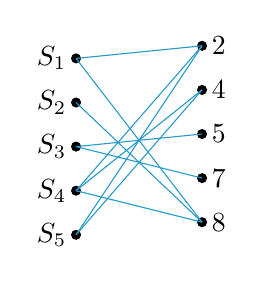
\begin{tikzpicture}[scale=0.8]
    % Sets
    \foreach \i in {1,...,5} \coordinate (s\i) at (0, 3 - 0.7*\i);
    \node[left] at (s1) {$S_1$}; \node[left] at (s2) {$S_2$}; \node[left] at (s3) {$S_3$};
    \node[left] at (s4) {$S_4$}; \node[left] at (s5) {$S_5$};
    \foreach \i in {1,...,5} \filldraw (s\i) circle (2pt);
    
    % Elements
    \coordinate (e2) at (2, 2.5); \node[right] at (e2) {2};
    \coordinate (e4) at (2, 1.8); \node[right] at (e4) {4};
    \coordinate (e5) at (2, 1.1); \node[right] at (e5) {5};
    \coordinate (e7) at (2, 0.4); \node[right] at (e7) {7};
    \coordinate (e8) at (2, -0.3); \node[right] at (e8) {8};
    \foreach \e in {e2,e4,e5,e7,e8} \filldraw (\e) circle (2pt);
    
    % Edges based on containment
    \draw[cyan!80!black] (s1)--(e2); \draw[cyan!80!black] (s1)--(e8);
    \draw[cyan!80!black] (s2)--(e8);
    \draw[cyan!80!black] (s3)--(e5); \draw[cyan!80!black] (s3)--(e7);
    \draw[cyan!80!black] (s4)--(e2); \draw[cyan!80!black] (s4)--(e4); \draw[cyan!80!black] (s4)--(e8);
    \draw[cyan!80!black] (s5)--(e2); \draw[cyan!80!black] (s5)--(e4);
\end{tikzpicture}
\end{center}
With this visualisation the question translates into asking whether $\mathcal{F}$ is matched into $U = \cup S_i$.
Let $S = \{S_1, S_2, S_4, S_5\}$. Then $|S|=4$. On the other hand, $|N(S)| = |\{2,4,8\}| = 3$. So $|S| > |N(S)|$ and by Hall's marriage theorem, there is no system of distinct representatives for $\mathcal{F}$. If we consider $\mathcal{F}_0 := \{S_1, S_2, S_3, S_4\}$ however, then a system of distinct representatives is given by $\{2,8,5,4\}$.
\end{example}

% 7.15 Theorem
\begin{theorem}
Let $\mathcal{F}=\{S_1, S_2, \dots, S_k\}$ be a family of nonempty sets. Then $\mathcal{F}$ has a system of representatives iff for any $I \subseteq \{1, 2, \dots, k\}$ we have that $|I| \le |\cup_{i \in I} S_i|$.
\end{theorem}

\begin{proof}
Exercise, easy consequence from Hall's marriage theorem.
\end{proof}

\section{The K\"{o}nig-Egerv\'{a}ry Theorem}
We want to finish the chapter on matchings by relating them to yet another very important graph concept - the one of vertex covers.

% 7.16 Definition
\begin{definition}
Let $G$ be a graph. A \textbf{\color{red}vertex cover} for $G$ is a vertex set $C \subseteq V(G)$ s.t. every edge of $G$ has at least one endvertex in $C$, i.e. $\forall e \in E(G) \exists x \in C \text{ s.t. } x \in e$.\\
A vertex cover is called a \textbf{\color{red}minimum vertex cover} if there is no vertex cover of smaller cardinality.
\end{definition}

% 7.17 Application
\topic{Application}
Imagine a museum with many galleries. We want to position guards within the galleries that have all art pieces in sight. If we model galleries as edges and places where at least two galleries meet as vertices, then we obtain a graph. Now every vertex cover for $G$ would provide an appropriate list of locations to place our guards. Of course, we want to minimize our spendings when usually we are interested in finding a minimum vertex cover.

% 7.18 Remark
\begin{remark}
\begin{enumerate}
    \item[1)] Every graph $G$ has a vertex cover, namely $V_G$.
    \item[2)] If $C$ is a vertex cover for $G$ and $C \subseteq D$, then $D$ is a vertex cover for $G$.
\end{enumerate}
\end{remark}

% 7.19 Example
\begin{example}
Consider $G$ given by
\begin{center}
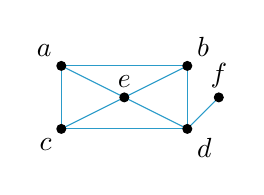
\begin{tikzpicture}[scale=0.8]
    \coordinate (c) at (0,0); \coordinate (d) at (2,0);
    \coordinate (a) at (0,1); \coordinate (b) at (2,1);
    \coordinate (e) at (1, 0.5); \coordinate (f) at (2.5,0.5);
    
    \draw[cyan!80!black] (a)--(b)--(d)--(c)--(a);
    \draw[cyan!80!black] (a)--(e); \draw[cyan!80!black] (b)--(e); \draw[cyan!80!black] (c)--(e); \draw[cyan!80!black] (d)--(e);
    \draw[cyan!80!black] (d)--(f);

    \foreach \p in {a,b,c,d,e,f} \filldraw (\p) circle (2pt);
    
    \node[above left] at (a) {$a$}; \node[above right] at (b) {$b$};
    \node[below left] at (c) {$c$}; \node[below right] at (d) {$d$};
    \node[above] at (e) {$e$};
    \node[above] at (f) {$f$};
\end{tikzpicture}
\end{center}
Then one vertex cover is given by $C_1 := \{a,b,c,d\}$. But also, $C_2 := \{a,e,d\}$ is a vertex cover of smaller cardinality. It is not hard to see that there is no vertex cover containing only two vertices, whence $C_2$ is minimal.
\end{example}


% 7.20 Lemma
\begin{lemma}
Let $G$ be a graph, $M$ any matching for $G$ and $C$ any vertex cover for $G$. Then $|M| \le |C|$. In particular, a maximum matching contains at most as many edges as a minimal vertex cover contains vertices.
\end{lemma}

\begin{proof}
Let $M$ be any matching for $G$, say $M=\{e_1, e_2, \dots, e_k\}$, and $C$ any vertex cover. For any $e_i \in M$ there is a vertex $x_i \in C$ incident with $e_i$. As all $e_i$'s are disjoint, all the $x_1, x_2, \dots, x_k$ are distinct. Thus, $C$ contains at least as many elements as $M$, i.e. $|M| \le |C|$. \qedhere
\end{proof}

Now, what changes if we restrict ourselves to bipartite graphs? Somehow we have more control over the relation between vertices and edges. Indeed, the Hungarian mathematicians D\'{e}nes K\"{o}nig and Jen\H{o} Egerv\'{a}ry independently discovered the following in 1931.

% 7.21 Theorem (Konig-Egervary)
\begin{theorem}[König-Egerváry]
Let $G$ be a bipartite graph. Then any maximum matching has the same cardinality as any minimum vertex cover.
\end{theorem}

\begin{proof}
Consider an arbitrary bipartite graph $G$ and a maximum matching $M$.
We will show that there exists a vertex cover $C$ s.t. $|M|=|C|$.
By Lemma 7.20, $C$ then is a minimum vertex cover. Let $X$ and $Y$ form a bipartition of $V_G$.

\vspace{0.3cm}
If every $x \in X$ is $M$-saturated, then $|X|=|M|$. Clearly, as $G$ is bipartite, the set $C:=X$ is a vertex cover for $G$, whence $|C|=|X|=|M|$ is as desired.

\vspace{0.3cm}
Now, assume \underline{not} every $x \in X$ is $M$ saturated.
Let $U := \{x \in X \mid x \text{ is not } M\text{-saturated}\}$. Then $|M|+|U| = |X|$. (*)

Similar to Hall's Lemma, set
\[ A := \{ v \in V(G) \mid \text{ex. an } M\text{-alternating } uv\text{-path for some } u \in U \}. \]
Further, set $S := A \cap X$ and $T := A \cap Y$. We claim that
\[ C := (X \setminus S) \cup T \text{ is a vertex cover with } |C|=|M|. \]

Exactly as in the proof of 7.12, we can show that
\begin{enumerate}
    \item[1)] Every vertex in $(S \setminus U) \cup T$ is $M$-saturated.
    \item[2)] $|S \setminus U| = |T|$.
    \item[3)] $T = N(S)$.
\end{enumerate}

Thus, we immediately get that $|T| = |S| - |U|$ (**) and thus
\begin{align*}
    |C| = |X \setminus S| \cup |T| &\overset{X \cap T = \emptyset}{=} |X \setminus S| + |T| \\
    &\overset{S \subseteq X}{=} |X| - |S| + |T| \\
    &\overset{(**)}{=} |X| - |S| + |S| - |U| \\
    &= |X| - |U| \overset{(*)}{=} |M|, \text{ as desired.}
\end{align*}

It remains to show that $C$ is a vertex cover for $G$.
To this end, let $e=xy$ be an arbitrary edge with $x \in X, y \in Y$. We need to show that at least one of $x$ or $y$ is in $C=(X \setminus S) \cup T$.
If $x \notin S$, i.e. $x \in X \setminus S$, we are done. Otherwise $x \in S$, whence $y \in N(S) = T$, as desired. This finishes the proof.
\end{proof}